\documentclass[conference]{IEEEtran}
\renewcommand{\IEEEkeywordsname}{Keywords}
\IEEEoverridecommandlockouts
% The preceding line is only needed to identify funding in the first footnote. If that is unneeded, please comment it out.
\usepackage[round,authoryear]{natbib}
\usepackage{amsmath,amssymb,amsfonts}
\usepackage{algorithmic}
\usepackage{graphicx}
\usepackage{balance}
\usepackage{textcomp}
\usepackage{float}
\usepackage{cuted}
\usepackage{caption}
\usepackage{placeins}
\captionsetup[figure]{font=footnotesize}
\usepackage{xcolor}
\usepackage{tikz}
\usepackage{pifont}
\usetikzlibrary{arrows.meta,positioning,calc,fadings,fit,backgrounds}
\usepackage{booktabs}
\usepackage[colorlinks=true, citecolor=blue, linkcolor=blue, urlcolor=blue]{hyperref}
\def\BibTeX{{\rm B\kern-.05em{\sc i\kern-.025em b}\kern-.08em
    T\kern-.1667em\lower.7ex\hbox{E}\kern-.125emX}}
\begin{document}
\title{CliniFusion-X: A Multimodal Clinical Intelligence
Framework for Chest X-ray Disease Diagnosis and
Reasoning\\
\thanks{}
}
\author{{\small\setlength{\tabcolsep}{3pt}\begin{tabular}{ccc}
\begin{minipage}[t]{0.32\textwidth}\centering
\textbf{K. Vishal Reddy}\\
\textit{Department of Computer Science and Engineering}\\
\mbox{\footnotesize\textit{Keshav Memorial Institute of Technology}}\\
Hyderabad 500029, Telangana, India\\
Kasarlavishalreddy@gmail.com
\end{minipage}
&
\begin{minipage}[t]{0.32\textwidth}\centering
\textbf{Gurram Vikramadithya}\\
\textit{Department of Computer Science and Engineering}\\
\mbox{\footnotesize\textit{Keshav Memorial Institute of Technology}}\\
Hyderabad 500029, Telangana, India\\
vikramadithya176@gmail.com
\end{minipage}
&
\begin{minipage}[t]{0.32\textwidth}\centering
\textbf{Periketi Ramu}\\
\textit{Department of Computer Science and Engineering}\\
\mbox{\footnotesize\textit{Keshav Memorial Institute of Technology}}\\
Hyderabad 500029, Telangana, India\\
periketiramu524@gmail.com
\end{minipage}
\\\noalign{\vskip 1em}
\begin{minipage}[t]{0.32\textwidth}\centering
\textbf{Saket Ausekar}\\
\textit{Department of Computer Science and Engineering}\\
\mbox{\footnotesize\textit{Keshav Memorial Institute of Technology}}\\
Hyderabad 500029, Telangana, India\\
saketausekar@gmail.com
\end{minipage}
&
\begin{minipage}[t]{0.32\textwidth}\centering
\textbf{Gopi Reddy Guru Lohith Reddy}\\
\textit{Department of Computer Science and Engineering}\\
\mbox{\footnotesize\textit{Keshav Memorial Institute of Technology}}\\
Hyderabad 500029, Telangana, India\\
gurulohith4582@gmail.com
\end{minipage}
&
\begin{minipage}[t]{0.32\textwidth}\centering
\textbf{Yeshamalla Vinay}\\
\textit{Department of Computer Science and Engineering}\\
\mbox{\footnotesize\textit{Keshav Memorial Institute of Technology}}\\
Hyderabad 500029, Telangana, India\\
tejv0001432@gmail.com
\end{minipage}
\end{tabular}
}}
\maketitle
\begin{abstract}
Chest X-ray imaging is widely used to examine thoracic diseases because it is accessible, inexpensive, and non-invasive. Automatic analysis is challenging when multiple abnormalities coexist, diseases have similar appearances or the findings occupy small or subtle regions. Image-only approaches also lack the structured clinical information typically available for the patient. We propose CliniFusion-X, an explainable multimodal framework that combines chest X-ray images and structured clinical information for multi-label thoracic disease analysis. A Swin Transformer extracts hierarchical visual representations to predict multiple findings in a single radiograph, complemented by patient-related clinical context. We compare this visual model with a DINOv2-based model using shallow CNN feature refinement on the same multi-label task. The experiments show better overall performance for the Swin Transformer, while Score-CAM provides interpretable evidence by highlighting visually relevant regions associated with its predictions.
\end{abstract}
\begin{IEEEkeywords}
Chest X-ray, Multi-Label Classification, Swin Transformer, DINOv2, CNN, Clinical Consistency Module, Score-CAM
\end{IEEEkeywords}
\section{INTRODUCTION}
The X-ray imaging of the chest is a routine tool for the diagnosis of thoracic diseases because it is quickly obtained, usually available and cost effective. Many different thoracic diseases can be diagnosed on a chest X-ray including pneumonia, cardiomegaly, pleural effusion and pneumothorax and other diseases \citep{wang2017chestxray8}. The interpretation is challenging because diseases can share visual patterns, overlapping anatomy can lead to abnormal findings and findings may occupy small or low-contrast regions. Multiple abnormalities in a single radiograph further complicate identification, requiring careful examination.

In the analysis of chest X-rays, for example convolutional neural networks (CNNs) are used to learn a variety of disease-related features like edges, textures, shapes. However, these networks are less suited to learning relationships between distant parts of the image. The abnormal locations can provide useful information for classification, particularly for findings in specific anatomical regions \citep{guendel2018location}. Detecting multiple diseases also motivates approaches that learn relationships between findings \citep{pham2021interpreting}.

Vision Transformer (ViT) learns dependencies through self-attention
between image regions to capture the global context.
DINOv2 learns high-level visual representations using self-
supervised learning on large image data using large-scale image data, using a shallow CNN available to refine local features \citep{oquab2023dinov2}. In contrast, the Swin Transformer uses a hierarchical design with local and shifted attention windows \citep{liu2021swin}. These different representations motivate their comparison for multi-label thoracic disease analysis.

We propose CliniFusion-X, an explainable multimodal framework for multi-label thoracic disease analysis. The pretrained Swin Transformer is fine-tuned on chest X-rays to adapt visual representations to medical imaging, while structured clinical information adds patient context. A DINOv2 model with shallow CNN feature refinement is independently evaluated on the same task as a comparative model. Score-CAM provides visual explanations to support understanding of the predictions \citep{wang2020scorecam}.
\section{LITERATURE REVIEW}
\citet{baltruschat2019comparison} compared deep learning approaches for multi-label chest X-ray classification, examining transfer learning, fine-tuning, and age and gender information and its results stressed about model selection and information beyond images.

\citet{allaouzi2019multilabel} studied CNN feature extraction and problem-transformation methods on ChestX-ray14 and CheXpert. CliniFusion-X also employs a multi-label setup and patient information.

These studies have been based on multi-label datasets. \citet{irvin2019chexpert} introduced CheXpert, a big set of chest X-rays with expert comparison and uncertainty labels. \citet{nguyenmau2023longtailed} studied data augmentation and ensembling strategies for long-tailed multi-label chest X-ray classification. Our work handles class imbalance by positive-class weighting.

\citet{holste2024cxrlt} presented CXR-LT a multi-label, multi-institutional and multi-findings chest X-ray classification task with significant long-tailed class imbalance. \citet{wang2024multilabel} combined local awareness and global co-occurrence to consider local image properties and relations between findings. These works motivate us in terms of class imbalance handling and multi-label strategies.

\citet{swinchex2022} designed SwinCheX, a Swin Transformer with an MLP classification head, reporting promising results for multi-label ChestX-ray14. CliniFusion-X improves upon the visual modality by including structured clinical information and a Clinical Consistency Module to consider patient context related to the prediction of the disease.

\citet{fu2025davit} developed DAViT, a domain adapted Vision Transformer for chest X-ray pneumonia detection and explanation. CliniFusion-X adapts pretrained visual representations by fine-tuning. However, it is applied to multi-label thoracic disease classification and includes structured clinical data.

\citet{aksoy2024beyond} combined structured patient data and chest X-rays for report generation, showing the added value of information outside the image. CliniFusion-X considers patient information as well as final image predictions by the Clinical Consistency Module. It also uses Wang et al.'s Score-CAM \citep{wang2020scorecam}, a gradient-free method for class-specific explanations, to visualize the relevant image regions for the predicted findings.

\citet{singh2025chestxtranscribe} developed ChestX-Transcribe, a multimodal Transformer model for report generation in radiology. These helped us to the add value of interpretability and additional information in medical AI as a clinical report.

{\tolerance=2000\emergencystretch=3em
CAM-CheX introduces the clinical data alongside chest X-ray images for multi-label thoracic disease classification which motivated us for generating the clinical report \citep{pmlr-v297-sloan26a}.
All these works together show the added value of patient data during report generation. The visual representation, multi-label classification, class imbalance, clinical information and interpretability have generally been handled independently in the literature, rather than in one multi-label model for thoracic diseases. CliniFusion-X combines Swin representations, structured clinical data, class imbalance handling and Score-CAM explanations, with an independent DINOv2 + CNN comparator.\par}
\begin{strip}
    \noindent\begin{minipage}{\columnwidth}
        \section{PROPOSED ARCHITECTURE MODEL}
    \end{minipage}\par\medskip
    \centering
    \resizebox{\textwidth}{!}{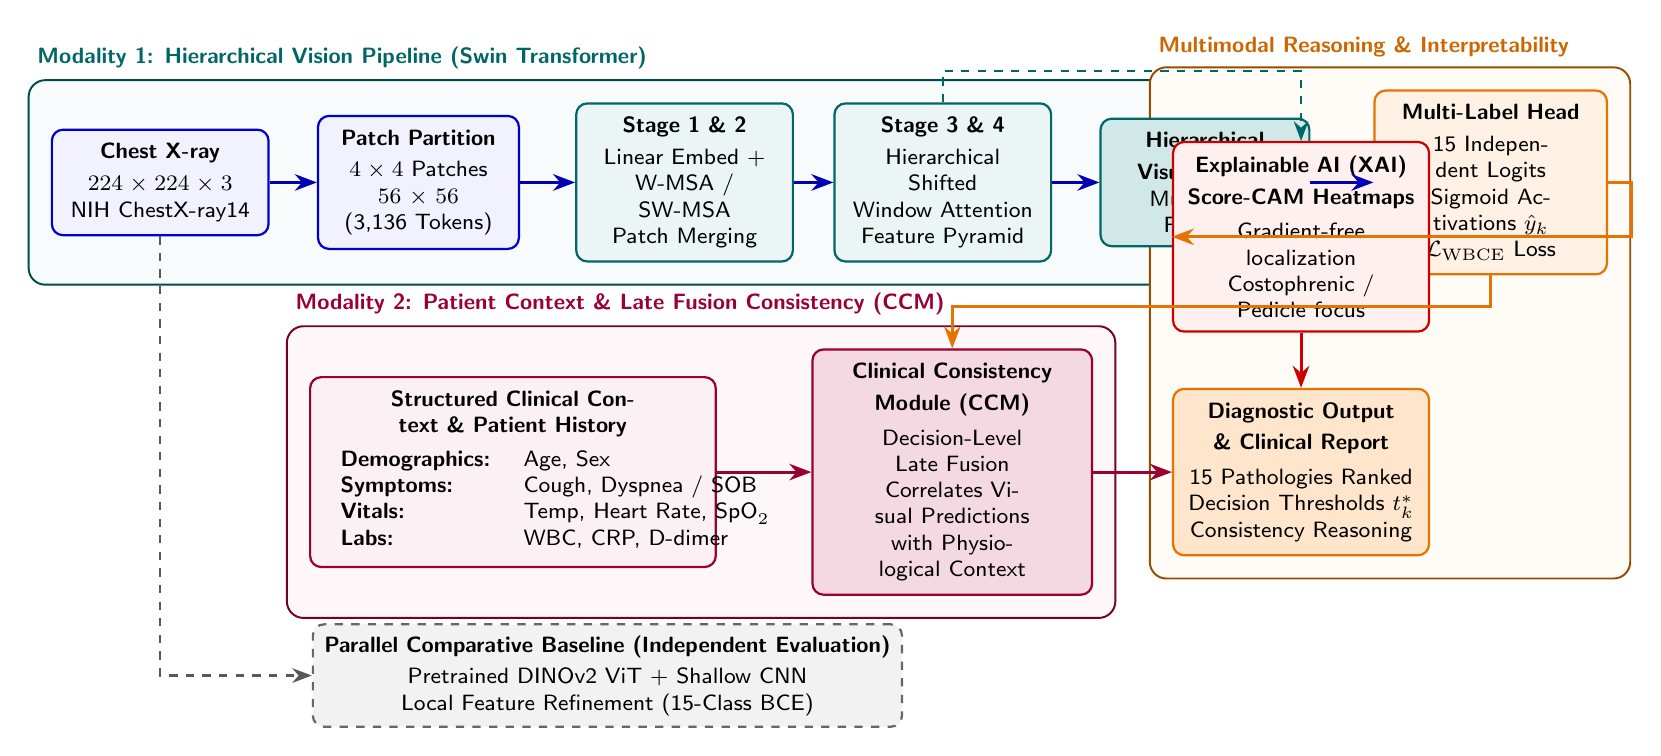
\begin{tikzpicture}[
    >=Stealth,
    node distance=0.8cm and 0.9cm,
    font=\sffamily\footnotesize,
    % Styles
    box/.style={
        draw=blue!80!black, 
        fill=blue!5, 
        rounded corners=4pt, 
        line width=0.8pt, 
        align=center, 
        inner sep=5pt
    },
    swinbox/.style={
        draw=teal!80!black, 
        fill=teal!8, 
        rounded corners=4pt, 
        line width=0.8pt, 
        align=center, 
        inner sep=5pt
    },
    clinbox/.style={
        draw=purple!80!black, 
        fill=purple!6, 
        rounded corners=4pt, 
        line width=0.8pt, 
        align=center, 
        inner sep=5pt
    },
    headbox/.style={
        draw=orange!90!black, 
        fill=orange!10, 
        rounded corners=4pt, 
        line width=0.8pt, 
        align=center, 
        inner sep=5pt
    },
    xaibox/.style={
        draw=red!80!black, 
        fill=red!6, 
        rounded corners=4pt, 
        line width=0.8pt, 
        align=center, 
        inner sep=5pt
    },
    dinobox/.style={
        draw=gray!80!black, 
        fill=gray!10, 
        rounded corners=4pt, 
        dashed, 
        line width=0.8pt, 
        align=center, 
        inner sep=4pt
    },
    grouppanel/.style={
        draw=#1!60!black, 
        fill=#1!3, 
        rounded corners=6pt, 
        line width=0.7pt, 
        inner sep=8pt
    },
    header/.style={
        font=\sffamily\bfseries\footnotesize, 
        text=#1!80!black
    },
    flow/.style={
        ->, 
        line width=1.1pt, 
        draw=blue!70!black
    },
    flowdashed/.style={
        ->, 
        line width=0.9pt, 
        dashed, 
        draw=gray!70!black
    },
    flowpink/.style={
        ->, 
        line width=1.1pt, 
        draw=purple!80!black
    },
    floworange/.style={
        ->, 
        line width=1.1pt, 
        draw=orange!90!black
    }
]

% ==================== ROW 1: INPUTS ====================
% CXR Input
\node[box, text width=2.4cm] (cxr) {
    \textbf{Chest X-ray}\\[2pt]
    $224 \times 224 \times 3$\\
    NIH ChestX-ray14
};

% Patch Partition
\node[box, right=0.6cm of cxr, text width=2.2cm] (patch) {
    \textbf{Patch Partition}\\[2pt]
    $4 \times 4$ Patches\\
    $56 \times 56$ (3,136 Tokens)
};

% Swin Stages
\node[swinbox, right=0.7cm of patch, text width=2.4cm] (swin1) {
    \textbf{Stage 1 \& 2}\\[2pt]
    Linear Embed + \\
    W-MSA / SW-MSA\\
    Patch Merging
};

\node[swinbox, right=0.5cm of swin1, text width=2.4cm] (swin2) {
    \textbf{Stage 3 \& 4}\\[2pt]
    Hierarchical Shifted\\
    Window Attention\\
    Feature Pyramid
};

% Visual Representation Vector
\node[swinbox, right=0.6cm of swin2, text width=2.3cm, fill=teal!18] (visfeat) {
    \textbf{Hierarchical}\\[2pt]
    \textbf{Visual Vector}\\
    Multi-Scale Features
};

% ==================== MULTI-LABEL HEAD ====================
\node[headbox, right=0.8cm of visfeat, text width=2.6cm] (mlhead) {
    \textbf{Multi-Label Head}\\[2pt]
    15 Independent Logits\\
    Sigmoid Activations $\hat{y}_k$\\
    $\mathcal{L}_{\mathrm{WBCE}}$ Loss
};

% ==================== CLINICAL INFORMATION ====================
\node[clinbox, below=1.6cm of patch, text width=4.8cm, xshift=1.2cm] (clinical) {
    \textbf{Structured Clinical Context \& Patient History}\\[3pt]
    \begin{tabular}{ll}
    \textbf{Demographics:} & Age, Sex \\
    \textbf{Symptoms:} & Cough, Dyspnea / SOB \\
    \textbf{Vitals:} & Temp, Heart Rate, $\text{SpO}_2$ \\
    \textbf{Labs:} & WBC, CRP, D-dimer
    \end{tabular}
};

% ==================== CLINICAL CONSISTENCY MODULE (CCM) ====================
\node[clinbox, right=1.2cm of clinical, text width=3.2cm, fill=purple!15] (ccm) {
    \textbf{Clinical Consistency}\\[2pt]
    \textbf{Module (CCM)}\\[3pt]
    Decision-Level Late Fusion\\
    Correlates Visual Predictions\\
    with Physiological Context
};

% ==================== FINAL OUTPUT & REPORT ====================
\node[headbox, right=1.0cm of ccm, text width=2.9cm, fill=orange!20] (report) {
    \textbf{Diagnostic Output}\\[2pt]
    \textbf{\& Clinical Report}\\[3pt]
    15 Pathologies Ranked\\
    Decision Thresholds $t_k^*$\\
    Consistency Reasoning
};

% ==================== XAI SCORE-CAM ====================
\node[xaibox, above=0.7cm of report, text width=2.9cm] (scorecam) {
    \textbf{Explainable AI (XAI)}\\[2pt]
    \textbf{Score-CAM Heatmaps}\\[3pt]
    Gradient-free localization\\
    Costophrenic / Pedicle focus
};

% ==================== COMPARATIVE MODEL (DINOv2 + CNN) ====================
\node[dinobox, below=0.7cm of clinical, text width=7.2cm, xshift=1.2cm] (dino) {
    \textbf{Parallel Comparative Baseline (Independent Evaluation)}\\[2pt]
    Pretrained DINOv2 ViT + Shallow CNN Local Feature Refinement (15-Class BCE)
};

% ==================== CONNECTIONS / FLOWS ====================
\draw[flow] (cxr) -- (patch);
\draw[flow] (patch) -- (swin1);
\draw[flow] (swin1) -- (swin2);
\draw[flow] (swin2) -- (visfeat);
\draw[flow] (visfeat) -- (mlhead);

% Head to CCM
\draw[floworange] (mlhead.south) -- ++(0,-0.4) -| (ccm.north);

% Head to Score-CAM
\draw[floworange] (mlhead.east) -- ++(0.3,0) |- (scorecam.west);

% Clinical to CCM
\draw[flowpink] (clinical.east) -- (ccm.west);

% CCM to Report
\draw[flowpink] (ccm.east) -- (report.west);

% Score-CAM to Report
\draw[->, draw=red!80!black, line width=1.1pt] (scorecam.south) -- (report.north);

% Visual to Score-CAM
\draw[->, draw=teal!80!black, dashed, line width=0.9pt] (swin2.north) -- ++(0,0.4) -| (scorecam.north);

% DINO comparison indicator
\draw[flowdashed] (cxr.south) |- (dino.west);

% Background panels/labels
\begin{scope}[on background layer]
    % Visual extraction group
    \node[grouppanel=teal, fit=(cxr) (patch) (swin1) (swin2) (visfeat)] (g1) {};
    \node[header=teal, anchor=south west] at (g1.north west) {Modality 1: Hierarchical Vision Pipeline (Swin Transformer)};

    % Clinical context group
    \node[grouppanel=purple, fit=(clinical) (ccm)] (g2) {};
    \node[header=purple, anchor=south west] at (g2.north west) {Modality 2: Patient Context \& Late Fusion Consistency (CCM)};

    % Output group
    \node[grouppanel=orange, fit=(mlhead) (scorecam) (report)] (g3) {};
    \node[header=orange, anchor=south west] at (g3.north west) {Multimodal Reasoning \& Interpretability};
\end{scope}

\end{tikzpicture}
}

    \captionof{figure}{
    Overall Architecture of CliniFusion-X: A Multimodal Clinical Intelligence Framework for Chest X-ray Diagnosis with Explainable AI.
    }
    \label{fig:architecture}
\end{strip}
The CliniFusion-X formulates chest X-ray analysis as multi-label classification, independently predicting each target label rather than assigning a single class, because multiple thoracic abnormalities can coexist.

The Fig.~\ref{fig:architecture} methodology has several phases, starting from the NIH ChestX-ray14 preparation,
image preprocessing then class imbalance handling is addressed and fed into the Swin Transformer for 
feature extraction and integrated with structured clinical information and followed by multi-label classification using the combined representation. DINOv2 with shallow CNN refinement provides a comparative model, and Score-CAM explains the predictions over highlighted regions.
\subsection{\textbf{Dataset and Pre-processing}}
Experiments are performed on the NIH ChestX-ray14 dataset which contains 112,120 images from 30,805 unique patients with patient ID, age, gender, and finding labels. Images can contain multiple findings of diseases, so our 15-label taxonomy includes 14 thoracic findings and a No Finding category. The Patient-disjoint splits prevent patient-level leakage, with multi-label stratification maintaining reasonable distributions across approximately 70\% training, 15\% validation, and 15\% test images. Images were resized to $256 \times 256$ and normalized with ImageNet statistics. Training used random $224 \times 224$ crops, horizontal flipping, and $\pm5^\circ$ rotation, validation and testing used $224 \times 224$ center crops without augmentation.
\subsection{\textbf{Handling Class Imbalance}}
The positive samples are not evenly distributed among different findings of the dataset, with some conditions have far fewer positive samples than others. To address this imbalance, Binary Cross-Entropy with Logits loss and positive-class weighting was used, for each label the binary cross-entropy is
\begin{equation}
\mathcal{L}_{\mathrm{BCE}}
=
-\left[
y\log(\hat{y})
+
(1-y)\log(1-\hat{y})
\right].
\end{equation}
where $y$ is the true label and $\hat{y}$ the predicted probability. A positive-class weight $w_p$ emphasizes underrepresented positive samples:
\begin{equation}
\mathcal{L}_{\mathrm{WBCE}}
=
-\left[
w_p y\log(\hat{y})
+
(1-y)\log(1-\hat{y})
\right].
\end{equation}
The weights are derived from training class frequencies and limited to a predefined range to prevent large values from dominating training. Loss is computed independently for all 15 labels. The training uses AdamW with learning rate \(1\times10^{-4}\) and weight decay \(1\times10^{-4}\).
\subsection{\textbf{Swin Transformer Architecture}}
The main visual feature extractor of CliniFusion-X is Swin-Tiny, initialized with ImageNet pretrained weights and fine-tuned on chest X-rays using configuration called \textsf{swin\_tiny\_patch4\_window7\_224}.
The model takes a $224 \times 224$ input image and divides into $4 \times 4$ non-overlapping regions to create patches. This gives 56 patches of each dimension and thus 3,136 initial patches. Their feature representations pass through the hierarchical architecture that is the Swin Transformer and it performs self attention in local window rather than whole-image. Each patch will be processed through two different types of attention layers that are  Window-based Multi Head Self Attention (W-MSA) and Shifted Window based Multi Head Self Attention (SW-MSA). Shifted windows exchange information between neighboring regions assigned to different windows in the preceding block. Attention is defined as
\begin{equation}
\operatorname{Attention}(Q,K,V)
=
\operatorname{Softmax}
\left(
\frac{QK^T}{\sqrt{d}}
\right)V,
\end{equation}
where $Q$, $K$, and $V$ are the query, key, and value representations and $d$ is the dimension of the key vectors.
The Patch Merging between stages reduces spatial resolution and increases feature dimension of progressing from fine-grained local to higher-level representations. This hierarchy accommodates abnormalities at different spatial scales.
\subsection{\textbf{Clinical Data and Patient History}}
The interface enables the user to view the chest X-ray with the additional entry of structured clinical information such that patient details can be taken into account alongside the image. The fields are patient information (age and sex), symptoms (shortness of breath, cough), vital signs (temperature, heart rate, and SpO2) and laboratory data (WBC, CRP, and D-dimer). This may help to provide a more informed interpretation of model predictions.
\subsection{\textbf{Clinical Consistency Module (CCM)}}
The Clinical Consistency Module (CCM) checks predicted findings against user-provided clinical information and patient context. It is a decision-level late-fusion consistency layer integrating final image predictions with available clinical evidence at the pipeline's end and these helps to produce the overall clinical report.
\subsection{\textbf{Multi-Label Classification}}
To allow multiple findings in one radiograph, the classification head produces 15 independent logits, one per target label with independent sigmoid activation:
\begin{equation}
\hat{y}_k
=
\sigma(z_k)
=
\frac{1}{1+\exp(-z_k)},
\qquad k=1,\ldots,15.
\end{equation}
Here, $z_k$ is the output logit for the $k$-th label and $\hat{y}_k$ is its corresponding predicted probability. The independent sigmoid outputs can assign high probabilities to concurrent findings such as Cardiomegaly and Effusion, unlike softmax classification which generally assumes mutually exclusive classes.
\subsection{\textbf{Comparative Model: DINOv2 + CNN}}
A separate DINOv2 + CNN baseline combines self-supervised pretrained visual representations with global and shallow CNN refinement of local features. It is independently evaluated
on the same multi-label chest X-ray task to compare visual
representations and overall classification performance, and is
not integrated into the Swin-based CliniFusion-X model.
\subsection{\textbf{Explainable AI (XAI) Interpretation}}
Score-CAM produces a class-specific visual explanations for improving the interpretability of the model indicating the image areas relevant to the predicted findings in the interface contributing to model output. They provide visual evidence to support human understanding not substitute for clinical judgment.
\section{RESULTS AND DISCUSSION}
\subsection{Evaluation Metrics}
We evaluate the model on an independent test dataset by considering the problem as a multi-label classification problem. Evaluation would be done based on the measures such as Precision, Recall, F1-score and False Positive Rate. In addition, the study will also compute Receiver Operating Characteristic curves and Area Under ROC. The evaluation measures will be used to assess the performance of the models.
\subsubsection{Precision}
Precision represents the proportion of predicted positive cases that are actually positive. It is calculated as:
\begin{equation}
\mathrm{Precision}
=
\frac{TP}{TP+FP}
\end{equation}
A higher Precision indicates fewer false positive predictions.
\subsubsection{Recall and Sensitivity}
Recall is also referred to as Sensitivity or True Positive Rate (TPR) that represents the proportion of actual positive cases correctly identified by the model. It is calculated as:
\begin{equation}
\mathrm{Recall}
=
\mathrm{Sensitivity}
=
\frac{TP}{TP+FN}
\end{equation}
A higher Recall indicates that more positive cases are correctly detected.
\subsubsection{F1-Score}
The F1-score provides a balance between Precision and Recall. It is particularly useful for imbalanced classification problems because it considers both false-positive and false-negative predictions.
\begin{equation}
\mathrm{F1}
=
\frac{2\times\mathrm{Precision}\times\mathrm{Recall}}
{\mathrm{Precision}+\mathrm{Recall}}
\end{equation}
\subsubsection{False Positive Rate}
The False Positive Rate (FPR) represents the proportion of actual negative cases that are incorrectly classified as positive. It is calculated as:
\begin{equation}
\mathrm{FPR}
=
\frac{FP}{FP+TN}
\end{equation}
FPR is related to specificity, where a lower FPR corresponds to higher specificity.
\subsubsection{ROC and AUROC}
A ROC Curve and its Area Under the Curve (AUROC) illustrates how much of your True Positives you can get while minimizing your False Positives. The ROC curve is thus obtained by plotting TPR against FPR. Area under the ROC curve (AUROC) summarizes the ROC into a single value and is a function of the ability of the model to distinguish between the positive and negative case, across different thresholds. It can be expressed as:
\begin{equation}
\mathrm{AUROC}
=
\int_{0}^{1}
\mathrm{TPR}(u)\,
\mathrm{d}\mathrm{FPR}(u)
\end{equation}
A value closer to 1 indicates better discrimination, while a value around 0.5 indicates performance close to random classification.
For the multi-label problem, AUROC is calculated for individual disease labels and summarized using Macro AUROC and Micro AUROC.
\subsection{Threshold Selection}
The model outputs a probability between 0 and 1 for each disease label with the help of sigmoid activation function. The probability is then mapped to a classification threshold so helps to convert into a binary prediction. If the value is greater than or equal to the selected threshold then it is encountered as positive label or else negative. For example if the model predicts Cardiomegaly with a probability of 0.72 and selected threshold is 0.50 (in range from 0.05 to 0.95 for any disease), the prediction is considered as positive. Similarly, the probability of 0.32 and lower thresholds is negative. For each threshold, the obtained predictions are compared to the true labels to calculate TP, TN, FP, and FN. The acquired values are used to calculate Precision, Recall and F1-score. To determine the ideal threshold, various values may be employed to identify the one yielding the maximum F1-score.
\begin{table}[!htbp]
\caption{Example of Threshold Selection Using F1-Score}
\label{tab:threshold}
\centering
\renewcommand{\arraystretch}{1.1}
\begin{tabular}{cccc}
\hline
\textbf{Threshold} & \textbf{Precision} & \textbf{Recall} & \textbf{F1-Score} \\
\hline
0.20 & 0.60 & 0.71 & 0.65 \\
0.30 & 0.70 & 0.79 & 0.74 \\
0.40 & 0.76 & 0.81 & 0.78 \\
0.50 & 0.82 & 0.63 & 0.71 \\
\hline
\end{tabular}
\end{table}
The highest F1-score for this example is reached at a threshold of 0.40, as shown in Table~\ref{tab:threshold}. Thus, a threshold of 0.40 is selected for that particular disease label.
The best threshold for the $k$-th disease label is given by
\begin{equation}
t_k^{*}
=
\underset{t}{\operatorname{arg\,max}}
\;
\mathrm{F1}_k(t)
\end{equation}
where $t_k^{\star}$ is the threshold selected for the $k$-th disease label.
The threshold is determined using the validation set and then fixed for evaluation on the held-out test set. Since this is a multi-label classification problem, different disease labels may have different optimal thresholds.
\subsection{Overall Performance}
The overall performance of the two visual models is reported using Macro AUROC and Micro AUROC.
The Swin Transformer achieves a Macro AUROC of 0.8250 and a Micro AUROC of 0.8950, while the DINOv2 + CNN model achieves a Macro AUROC of 0.7885 and a Micro AUROC of 0.8417 under the reported experimental setting as shown in Table~\ref{tab:overall_performance}.
\begin{table}[H]
\caption{Overall Performance of the Visual Models}
\label{tab:overall_performance}
\centering
\renewcommand{\arraystretch}{1.1}
\begin{tabular}{lcc}
\hline
\textbf{Model} & \textbf{Macro AUROC} & \textbf{Micro AUROC} \\
\hline
DINOv2 + CNN & 0.7885 & 0.8417 \\
Swin Transformer & 0.8250 & 0.8950 \\
\hline
\end{tabular}
\end{table}
The higher AUROC values obtained by the Swin Transformer indicate better separation between positive and negative cases under the reported experimental setting. The difference can also be examined from the architectural perspective. The DINOv2 + CNN model combines high-level visual representations of DINOv2 with shallow CNN based local feature refinement and the Swin Transformer maintains shifted-hierarchical and window-based representations of window attention. This hierarchical design enables the Swin Transformer preserves fine-grained spatial information in early stages and build more general representations in deeper stages. This is relevant to chest X-ray analysis, as various findings may be at different spatial scales.
\subsection{Per-Class Performance}
The overall performance of the Swin Transformer and the comparative model 
DINOv2 + CNN on the basis of 15 target classes can be seen in the following results. They include the number of true positive samples, thresholds, AUROC, Precision, Recall, and F1-score for each class.
\begin{table*}[t]
\centering
\begin{minipage}[b]{0.45\textwidth}
\centering
\caption{Per-Class Performance of the Swin Transformer}
\label{tab:per_class_performance_swin}
\renewcommand{\arraystretch}{1.1}
\setlength{\tabcolsep}{2.5pt}
\scriptsize
\begin{tabular}{lrrrrrr}
\hline
\textbf{Class} & \textbf{Pos.} & \textbf{Thresh.} & \textbf{AUROC} & \textbf{Prec.} & \textbf{Rec.} & \textbf{F1} \\
\hline
Atelectasis         & 1807 & 0.74 & 0.8112 & 0.3333 & 0.4621 & 0.3873 \\
Cardiomegaly        & 390  & 0.74 & 0.8862 & 0.2587 & 0.3821 & 0.3085 \\
Consolidation       & 699  & 0.58 & 0.8013 & 0.1584 & 0.3662 & 0.2212 \\
Edema               & 348  & 0.75 & 0.8918 & 0.1919 & 0.3391 & 0.2451 \\
Effusion            & 2148 & 0.79 & 0.8827 & 0.4757 & 0.6345 & 0.5438 \\
Emphysema           & 398  & 0.63 & 0.9200 & 0.3580 & 0.4497 & 0.3987 \\
Fibrosis            & 255  & 0.39 & 0.8072 & 0.1566 & 0.1725 & 0.1642 \\
Hernia              & 30   & 0.48 & 0.8510 & 0.4242 & 0.4667 & 0.4444 \\
Infiltration        & 3166 & 0.60 & 0.7225 & 0.3737 & 0.4839 & 0.4217 \\
Mass                & 787  & 0.72 & 0.8334 & 0.3460 & 0.4282 & 0.3827 \\
No Finding          & 9369 & 0.42 & 0.7811 & 0.7021 & 0.8060 & 0.7504 \\
Nodule              & 953  & 0.61 & 0.7555 & 0.2438 & 0.3400 & 0.2840 \\
Pleural Thickening  & 553  & 0.67 & 0.7831 & 0.1955 & 0.2188 & 0.2065 \\
Pneumonia           & 209  & 0.51 & 0.7646 & 0.0592 & 0.1196 & 0.0792 \\
Pneumothorax        & 942  & 0.69 & 0.8831 & 0.4053 & 0.4883 & 0.4429 \\
\hline
\end{tabular}
\end{minipage}%
\hspace{0.05\textwidth}%
\begin{minipage}[b]{0.45\textwidth}
\centering
\caption{Per-Class Performance of DINOv2 + CNN}
\label{tab:per_class_performance_dino}
\renewcommand{\arraystretch}{1.1}
\setlength{\tabcolsep}{2.5pt}
\scriptsize
\begin{tabular}{lrrrrrr}
\hline
\textbf{Class} & \textbf{Pos.} & \textbf{Thresh.} & \textbf{AUROC} & \textbf{Prec.} & \textbf{Rec.} & \textbf{F1} \\
\hline
Atelectasis         & 1807 & 0.55 & 0.7612 & 0.2823 & 0.5932 & 0.3825 \\
Cardiomegaly        & 390  & 0.56 & 0.8721 & 0.3590 & 0.4113 & 0.3834 \\
Consolidation       & 699  & 0.56 & 0.7533 & 0.1706 & 0.4970 & 0.2540 \\
Edema               & 348  & 0.65 & 0.8373 & 0.2216 & 0.1708 & 0.1929 \\
Effusion            & 2148 & 0.69 & 0.8207 & 0.4162 & 0.7087 & 0.5244 \\
Emphysema           & 398  & 0.42 & 0.8775 & 0.2582 & 0.6331 & 0.3668 \\
Fibrosis            & 255  & 0.46 & 0.7929 & 0.1206 & 0.1885 & 0.1471 \\
Hernia              & 30   & 0.17 & 0.8269 & 0.0909 & 0.0116 & 0.0206 \\
Infiltration        & 3166 & 0.59 & 0.6957 & 0.3486 & 0.6904 & 0.4632 \\
Mass                & 787  & 0.68 & 0.8010 & 0.3227 & 0.4317 & 0.3693 \\
No Finding          & 9369 & 0.39 & 0.7310 & 0.5888 & 0.6378 & 0.6123 \\
Nodule              & 953  & 0.65 & 0.7381 & 0.2471 & 0.3220 & 0.2796 \\
Pleural Thickening  & 553  & 0.45 & 0.7526 & 0.1515 & 0.3377 & 0.2092 \\
Pneumonia           & 209  & 0.23 & 0.7127 & 0.0464 & 0.4193 & 0.0836 \\
Pneumothorax        & 942  & 0.56 & 0.8549 & 0.4205 & 0.5509 & 0.4770 \\
\hline
\end{tabular}
\end{minipage}
\end{table*}
\begin{figure*}[!t]
    \centering
    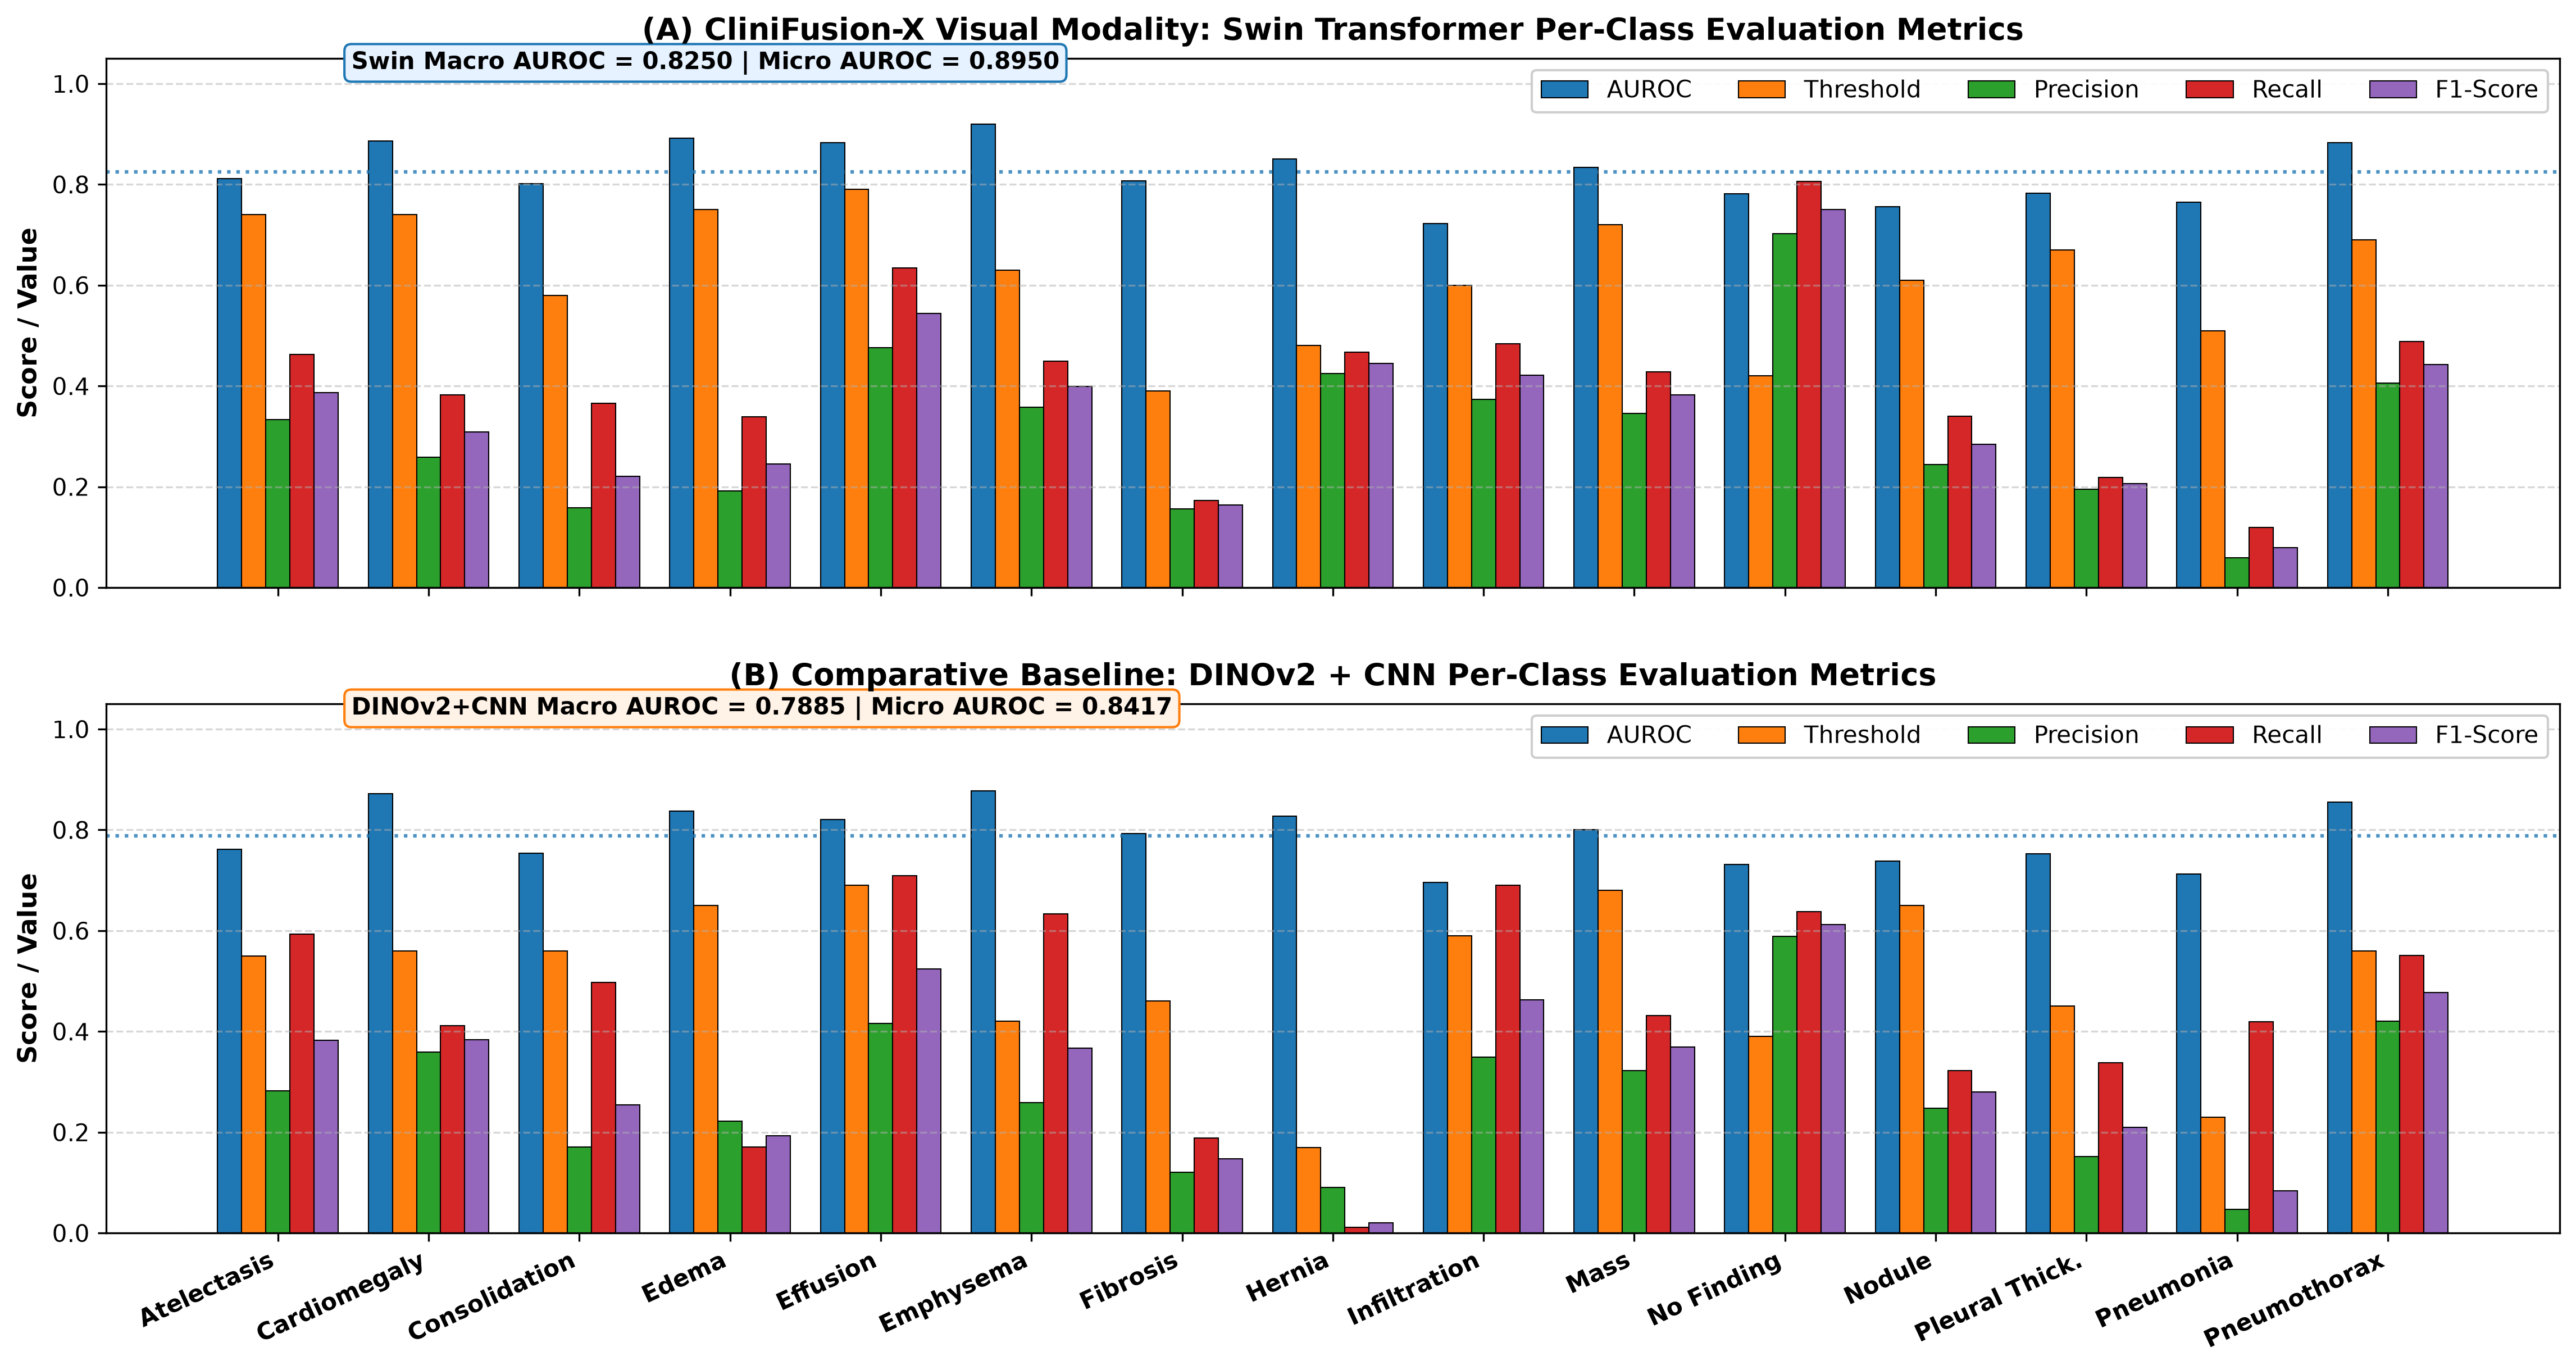
\includegraphics[
        width=\textwidth,
        keepaspectratio
    ]{Figure_2_Model_Comparison.png}
    
    \caption{Bar graph visualization of the per-class performance of the Swin Transformer and DINOv2 + CNN models in the 15 NIH ChestX-ray14 classes including AUROC, optimal thresholds, Precision, Recall and F1-score for each thoracic finding.}
    
    \label{fig:model_comparison}
\end{figure*}

The per-class results show that the model performs differently for different thoracic findings. This variation is expected in a multi-label and imbalanced dataset where the number of positive samples is significantly different in the classes. The results also emphasize the significance of class-specific threshold selection, as the optimal decision threshold is different for the disease categories. The detailed quantitative performance for each class is reported in Table~\ref{tab:per_class_performance_swin}, ~\ref{tab:per_class_performance_dino} and the comparative per-class results of the two visual models across all 15 ChestX-ray14 classes are shown in Fig.~\ref{fig:model_comparison} as a visualization format.


\subsection{Model Comparison}
The per-class performance of the Swin Transformer and DINOv2 + CNN models is compared across the 15 NIH ChestX-ray14 classes. The first row of the comparison presents the results of the Swin Transformer, while the second row presents the results of the DINOv2 + CNN model of the shown Fig.~\ref{fig:model_comparison}.
The DINOv2 + CNN model is evaluated independently on the same multi-label chest X-ray classification task. 
The comparison provides a basis for examining the differences between the hierarchical window-based representation of Swin Transformer and the pretrained visual representation with shallow CNN feature refinement used by DINOv2 + CNN.
\subsection{Explainability Analysis}
The Explainability Analysis offers more information about the image regions associated with the model predictions. Score-CAM was used to generate class-specific visual explanations for predicted thoracic findings.

The visual explanations highlight regions of the chest X-ray that contribute to individual model predictions. For example, the Effusion prediction mainly highlights regions around the costophrenic angles, whereas the Edema prediction shows higher activations around the vascular pedicle.
In the comparison, the DINOv2 + CNN model showed more diffuse activation patterns, while the Swin Transformer produced more directed visual responses in the highlighted regions. These visualizations provide additional information for examining the model predictions and the image regions contributing to the output.

\FloatBarrier
\section{CONCLUSION}
In this work we evaluate a Swin Transformer based strategy for multi-label
classification on a 15-label experimental taxonomy in chest X-ray
imaging. The method leverages hierarchical patch representations,
window-based self-attention, shifted windows and Patch Merging
to extract features at multiple spatial resolutions. A DINOv2-based model with shallow CNN feature refinement was also evaluated independently as a comparative visual approach.
The experimental results show that the Swin-based approach provides stronger overall discrimination than the evaluated DINOv2 + CNN configuration under the reported experimental setting. The hierarchical representation of the Swin Transformer allows visual information to be processed across different spatial scales, which is relevant to thoracic findings that can vary in size and location. The use of class-specific thresholds and positive-class weighting also supports the evaluation and handling of the multi-label and imbalanced nature of the dataset.
The framework also provides interpretable visual evidence through Score-CAM, allowing image regions contributing to predicted findings to be examined. In addition, the inclusion of structured clinical information and the Clinical Consistency Module provides patient-related context alongside the image-based predictions. These components support the understanding of model outputs while the final clinical interpretation remains with the medical professional.
Future work is going to look at how the framework performs differently in various hospitals and patient groups. Equipment variations are considered in imaging acquisition protocols and patient characteristics matter. That investigation will explore the framework's application as well. Medical imaging modalities like CT, which are three-dimensional, and MRI. This could be done in a manner that tests the method's applicability range to different clinical settings and types of medical images while still focusing on the framework's strengths in terms of human interpretability and the ability to facilitate human-in-the-loop analysis.

\balance
\makeatletter
\renewenvironment{thebibliography}[1]{%
\section*{REFERENCES}\footnotesize\raggedright\sloppy
\list{}{\labelwidth\z@\leftmargin1.5em\itemindent-1.5em\labelsep\z@
\itemsep0pt\parsep0pt\listparindent0pt\topsep0pt}%
\def\@biblabel##1{}%
\def\newblock{\hskip .11em plus .33em minus .07em}\sfcode`\.=1000\relax}{\endlist}
\makeatother
% APA 7th edition reference list (alphabetical by first author's surname)
\begin{thebibliography}{99}

\bibitem[Aksoy et al.(2024)]{aksoy2024beyond}
Aksoy, N., Sharoff, S., Baser, S., Ravikumar, N., \& Frangi, A. F. (2024).
Beyond images: An integrative multi-modal approach to chest X-ray report generation.
\textit{Frontiers in Radiology, 4}, Article 1339612.
\url{https://doi.org/10.3389/fradi.2024.1339612}

\bibitem[Allaouzi and Ben Ahmed(2019)]{allaouzi2019multilabel}
Allaouzi, I., \& Ben Ahmed, M. (2019).
A novel approach for multi-label chest X-ray classification of common thorax diseases.
\textit{IEEE Access, 7}, 64279--64288.
\url{https://doi.org/10.1109/ACCESS.2019.2916849}

\bibitem[Baltruschat et al.(2019)]{baltruschat2019comparison}
Baltruschat, I. M., Nickisch, H., Grass, M., Knopp, T., \& Saalbach, A. (2019).
Comparison of deep learning approaches for multi-label chest X-ray classification.
\textit{Scientific Reports, 9}, Article 6381.
\url{https://doi.org/10.1038/s41598-019-42294-8}

\bibitem[Fu et al.(2025)]{fu2025davit}
Fu, M., Tantithamthavorn, C., \& Le, T. (2025).
DAViT: A domain-adapted vision transformer for automated pneumonia detection and explanation using chest X-ray images.
\textit{IEEE Access, 13}, 103033--103044.
\url{https://doi.org/10.1109/ACCESS.2025.3579314}

\bibitem[Guendel et al.(2018)]{guendel2018location}
Guendel, S., Grbic, S., Georgescu, B., Zhou, K., Ritschl, L., Meier, A., \& Comaniciu, D. (2018).
Learning to recognize abnormalities in chest X-rays with location-aware dense networks.
\textit{arXiv}. \url{https://doi.org/10.48550/arXiv.1803.04565}

\bibitem[Holste et al.(2024)]{holste2024cxrlt}
Holste, G., Zhou, Y., Wang, S., Jaiswal, A., Lin, M., Zhuge, S., Yang, Y., Kim, D., Nguyen-Mau, T.-H., Tran, M.-T., Jeong, J., Park, W., Ryu, J., Hong, F., Verma, A., Yamagishi, Y., Kim, C., Seo, H., Kang, M., \ldots\ Peng, Y. (2024).
Towards long-tailed, multi-label disease classification from chest X-ray: Overview of the CXR-LT challenge.
\textit{Medical Image Analysis, 97}, Article 103224.
\url{https://doi.org/10.1016/j.media.2024.103224}

\bibitem[Irvin et al.(2019)]{irvin2019chexpert}
Irvin, J., Rajpurkar, P., Ko, M., Yu, Y., Ciurea-Ilcus, S., Chute, C., Marklund, H., Haghgoo, B., Ball, R., Shpanskaya, K., Seekins, J., Mong, D. A., Halabi, S. S., Sandberg, J. K., Jones, R., Larson, D. B., Langlotz, C. P., Patel, B. N., Lungren, M. P., \& Ng, A. Y. (2019).
CheXpert: A large chest radiograph dataset with uncertainty labels and expert comparison.
\textit{Proceedings of the AAAI Conference on Artificial Intelligence, 33}(1), 590--597.
\url{https://doi.org/10.1609/aaai.v33i01.3301590}

\bibitem[Liu et al.(2021)]{liu2021swin}
Liu, Z., Lin, Y., Cao, Y., Hu, H., Wei, Y., Zhang, Z., Lin, S., \& Guo, B. (2021).
Swin Transformer: Hierarchical vision transformer using shifted windows.
In \textit{Proceedings of the IEEE/CVF International Conference on Computer Vision (ICCV)} (pp. 10012--10022). IEEE.
\url{https://doi.org/10.1109/ICCV48922.2021.00986}

\bibitem[Nguyen-Mau et al.(2023)]{nguyenmau2023longtailed}
Nguyen-Mau, T.-H., Huynh, T.-L., Le, T.-D., Nguyen, H.-D., \& Tran, M.-T. (2023).
Advanced augmentation and ensemble approaches for classifying long-tailed multi-label chest X-rays.
In \textit{Proceedings of the IEEE/CVF International Conference on Computer Vision Workshops (ICCVW)} (pp. 2729--2738). IEEE.
\url{https://doi.org/10.1109/ICCVW60793.2023.00289}

\bibitem[Oquab et al.(2023)]{oquab2023dinov2}
Oquab, M., Darcet, T., Moutakanni, T., Vo, H., Szafraniec, M., Khalidov, V., Fernandez, P., Haziza, D., Massa, F., El-Nouby, A., Assran, M., Ballas, N., Galuba, W., Howes, R., Huang, P.-Y., Li, S.-W., Misra, I., Rabbat, M., Sharma, V., \ldots\ Bojanowski, P. (2023).
DINOv2: Learning robust visual features without supervision.
\textit{Transactions on Machine Learning Research}.
\url{https://doi.org/10.48550/arXiv.2304.07193}

\bibitem[Pham et al.(2021)]{pham2021interpreting}
Pham, H., Le, T., Tran, D. Q., Ngo, D., \& Nguyen, H. (2021).
Interpreting chest X-rays via CNNs that exploit hierarchical disease dependencies and uncertainty labels.
\textit{Neurocomputing, 437}, 186--194.
\url{https://doi.org/10.1016/j.neucom.2020.03.127}

\bibitem[Singh and Singh(2025)]{singh2025chestxtranscribe}
Singh, P., \& Singh, S. (2025).
ChestX-Transcribe: A multimodal transformer for automated radiology report generation from chest X-rays.
\textit{Frontiers in Digital Health, 7}, Article 1535168.
\url{https://doi.org/10.3389/fdgth.2025.1535168}

\bibitem[Sloan et al.(2026)]{pmlr-v297-sloan26a}
Sloan, P., Simpson, E., \& Mirmehdi, M. (2026).
Clinically-aligned multi-modal chest X-ray classification.
In \textit{Proceedings of the Fifth Machine Learning for Health Symposium} (Vol. 297, pp. 228--242). PMLR.
\url{https://doi.org/10.48550/arXiv.2511.09581}

\bibitem[Taslimi et al.(2022)]{swinchex2022}
Taslimi, S., Taslimi, S., Fathi, N., Salehi, M., \& Rohban, M. H. (2022).
SwinCheX: Multi-label classification on chest X-ray images with transformers.
\textit{arXiv}. \url{https://doi.org/10.48550/arXiv.2206.04246}

\bibitem[Wang et al.(2024)]{wang2024multilabel}
Wang, G., Wang, P., \& Wei, B. (2024).
Multi-label local awareness and global co-occurrence priori learning improve chest X-ray classification.
\textit{Multimedia Systems, 30}(3), Article 132.
\url{https://doi.org/10.1007/s00530-024-01321-z}

\bibitem[Wang et al.(2020)]{wang2020scorecam}
Wang, H., Wang, Z., Du, M., Yang, F., Zhang, Z., Ding, S., Mardziel, P., \& Hu, X. (2020).
Score-CAM: Score-weighted visual explanations for convolutional neural networks.
In \textit{Proceedings of the IEEE/CVF Conference on Computer Vision and Pattern Recognition Workshops (CVPRW)} (pp. 111--119). IEEE.
\url{https://doi.org/10.1109/CVPRW50498.2020.00020}

\bibitem[Wang et al.(2017)]{wang2017chestxray8}
Wang, X., Peng, Y., Lu, L., Lu, Z., Bagheri, M., \& Summers, R. M. (2017).
ChestX-ray8: Hospital-scale chest X-ray database and benchmarks on weakly-supervised classification and localization of common thorax diseases.
In \textit{Proceedings of the IEEE Conference on Computer Vision and Pattern Recognition (CVPR)} (pp. 2097--2106). IEEE.
\url{https://doi.org/10.1109/CVPR.2017.369}

\end{thebibliography}

\end{document}
